\documentclass{article}

\usepackage {amsmath}
\usepackage {setspace}
\usepackage [pdftex]{graphicx}
\usepackage[sort&compress]{achemso}
\usepackage{lineno}
\usepackage{textcomp}

% For typesetting roman numerals
\makeatletter
\newcommand{\rmnum}[1]{\romannumeral #1}
\newcommand{\Rmnum}[1]{\expandafter\@slowromancap\romannumeral #1@}
\makeatother

\usepackage[
top    = 1.0in,
bottom = 1.0in]{geometry}
% some formatting tags
%\oddsidemargin  0.0in
%\evensidemargin 0.0in
%\textwidth      6.5in

\title{Ab Initio Simulation Study of Malonic Acid
\author{Eric S. Shamay \and Geraldine L. Richmond}

\begin{document}


\newcommand{\ang}{\,$\textrm{\AA}$}
\newcommand{\angs}{\ang}
\newcommand{\wat}{H$_2$O}

%\maketitle

%\onehalfspacing
\linenumbers 
\doublespacing

\section {Introduction}

When we consider our recent experimental and theoretical achievements in studying simple organic acids in environmentally relevant systems, our scientific understanding remains poorly developed. The interfacial region of an aqueous solution is a turbulent and dynamic boundary where the behaviors of even small organic molecules evade definition. How does the liquid interfacial region alter behavior and strength of organic acid solutes? Do acid molecules interact with water at a surface as they do in bulk? What hydrate species and behavioral differences occur at an interface that are not found deeper in a liquid phase? Experiments addressing these types of questions give us valuable insight and information, but have not to date fully captured such microscopic behaviors and events. Computationally, however, these systems can be more fully characterized. Coupling computational results with previous experimental work provides a much more complete picture of acid behavior throughout aqueous interfacial regions.

Organic acids are a particularly interesting starting place for studying aqueous acid behavior. Dicarboxylic acids are a pertinent class of hygroscopic, water-soluble, and atmospherically relevant bolaamphiphilic molecules, receiving much attention in recent years both experimentally,\cite{Peng2001,Kawamura1993,Kawamura1996,Kawamura1996a,Kawamura1999,Senpere1994,Senpere1996,Aggarwal2008,Hsieh2007,Hsieh2009,Pavuluri2010,Nieminen1992,Nahalovsk1970,Dam1983,Mahiuddin2008,Odum1996,Odum1997,Pandis1991,Zhang1992,Hoffmann1997,Hori2003,Bilde2003,Nilsson1998} and in theoretical computational studies.\cite{Darvas2010,Darvas2011,Dlugosz2004,Mohajeri2004,Krijn1988,Chen2000,Nieminen1992,Mahiuddin2008,Ma2011,Nilsson1998} They vary in size from the smaller oxalic acid to larger humic-like substances.\cite{Chebbi1996,Badger2005} Dicarboxylic acids make up an appreciable amount of the atmospheric organic particulate matter, and are implicated in the nucleating condensation of clouds.\cite{Darvas2010,Darvas2011,Cruz1997,Zobrist2006,Hori2003,Shantz2003} Because of their presence in the atmosphere from biogenic and industrial processes, in various types of particulates and aerosols, they are known to affect climate conditions and atmospheric chemistry.\cite{Kanakidou2005,Finlayson-Pitts2000,Seinfeld1998,Darvas2010,Darvas2011,Zobrist2006,Yan2008,Odum1996,Odum1997,Pandis1991,Zhang1992,Hoffmann1997,Hori2003,Kawamura1996a,Bilde2003,Shantz2003} 

Malonic acid, the second-smallest of the dicarboxylic acids, has been studied in binary and heterogeneous reactions, and in aerosols to develop cloud nucleation models.\cite{Giebl2002,Finlayson-Pitts2009} It has previously been studied experimentally with several recent publications attesting to its importance.\cite{Parsons2004,Braban2003,Hansen2004,Hyvarinen2006,Riipinen2007} Many computational theoretical works have also probed the nature of malonic acid in small particles, at aqueous surfaces, and in gas phase.\cite{Nguyen2005,Merchan1984,Ma2011}

In this study we use ab initio molecular dynamics (MD) techniques to model and simulate the hydrating water structures that form around an interfacial malonic acid in water. The quantum MD technique described herein allows more realistic and accurate simulation than our previous classical MD study.\cite{Blower2012} In our previous work we determined net orientational behavior of malonic acid, coupled with experimental spectroscopic results to build a refined model of the acid's surface behavior. However, the classical interaction potential used needs to be tested against accurate quantum potentials to further verify the validity of the results obtained.

Quantum DFT MD simulation is the natural follow-up to the classical MD study as the interaction potential accurately reproduces hydration geometry around surface acid molecules. From the simulation data we examine in detail the specific bonding interactions that occur between surface waters and the carboxylic acid moieties of the malonic acid molecule, and look at the geometries and orientations of the hydrated acid molecule. Five concurrent simulations have been performed in this work, each of a malonic acid molecule bound to a water system surface. Each system was simulated at a temperature, solution concentration, and pH set to match the conditions of our most recent experimental studies.\cite{Blower2012} Our experiments showed that an aqueous malonic acid has a surface propensity in low-pH conditions. Although conclusions regarding the specific nature of those surface-bound hydrate complexes could only be inferred from experimental results, our previous and current computational simulations provide us with insights about the hydrated geometries of the acid molecules, and their orientational behavior.

We believe this computational study to be a necessary step in the development of models of malonic acid, and to continue building the picture of aqueous acid behavior. In this work we present a comparison between the classical and DFT interaction potentials to verify the validity of our previously used fully atomistic classical potential. We examine the internal geometry of surface malonic acid molecules, and discuss the behavioral implications of an interesting intramolecularly hydrogen-bonded species of malonic acid. These results complement several experimental and computational studies of the intramolecular interaction in several organic diacid conformers.\cite{Mohajeri2004,Dopieralski2011,Darvas2011,Nilsson1998,Chen2000,Eberson1959,Macoas2000,Macoas2000a,Merchan1984,Nguyen2005,Nieminen1992} We also show the orientational behavior of the aqueous surface acid molecule interacting with neighboring waters, specifying how the acid orients both with respect to the water surface, and internally by twisting about the carbone backbone bonds. Lastly, we analyze the vibrational behavior of the carbonyl modes of the acid to compare with, and complement our previous experimental results, and to further strengthen the link between our computational and experimental efforts.

\section {Computational Methods}

On-the-fly ab initio molecular dynamics simulations were performed with the QUICKSTEP package, which is an implementation of the Gaussian plane wave method using the Kohn-Sham formulation of density functional theory (DFT).\cite{VandeVondele2005} The Kohn-Sham orbitals are expanded using a linear combination of atom-centered Gaussian-type orbital functions. The electronic charge density was described using an auxiliary basis set of plane waves. Energies and forces from on-the-fly simulation sampling of the Born-Oppenheimer surface were calculated for each MD step using the Gaussian DZVP basis set, the exchange-correlation functional of Becke, Lee, Yang, and Parr (BLYP),\cite{LEE1988} and the atomic pseudo-potentials of the Goedecker, Teter, and Hutter type.\cite{Goedecker1996} A simulation timestep of 1 fs was used, with a Nose-Hoover thermostat set at 300K. These computational parameters were verified to yield a reasonable description of bulk room temperature water when simulating a neat-water system, and in our previous computational studies.\cite{Shamay2007}

Five equilibrated acid-water systems of size 10x10x15\angs were used in the simulations. Each system was initially randomly packed with 34 water molecules, and 2 HCl molecules. The system size was then expanded by 10\angs in the long cell dimension for final dimensions of 10x10x25\angs. A single malonic acid molecule was then added onto the top of the water phase within 2\angs of the topmost water molecule. The system energy was minimized through a geometry optimization procedure. Subsequently, the system was equilibrated for 1 ns in canonical ensemble (NVT) conditions. Periodic boundaries were set on all axes to form an infinite slab configuration. The equilibrated systems were then simulated for a further 30 ps in the microcanonical ensemble (NVE), with trajectory snapshots recorded every 1 fs. The initial 1 ns equilibration trajectory was not included in the final analysis. This simulation process resulted in 30,000 time steps of system trajectory for analysis in each replica of the system.
 

\include{Structure}
\section {Hydration Structure}

To compare the KS-DFT and classical interaction potentials, the O$_{mal}$-H$_{wat}$ radial distribution functions (RDF) are given in Figure \ref{fig:rdf} (where the subscripts ``mal'' refers to one of the malonic acid oxygens, and ``wat'' refers to water hydrogens). Both the KS-DFT (black) and classical (green) interaction potential RDFs are plotted in Figure \ref{fig:rdf}. The two RDFs shown are of the O$_{alcohol}$-H$_{wat}$ (left) and the O$_{carbonyl}$-H$_{wat}$ (right). There is reasonable agreement between the hydration structures calculated using the different interaction potentials. This is an indication that some features of the water packing around the carboxylic acid groups are reproduced in the classical potential in comparison with the KS-DFT interaction potential. Differences between the two interaction potentials appear mostly in the first solvation shell when looking at both the alcohol and carbonyl oxygen RDFs of Figure \ref{fig:rdf}. In the alcohol oxygen plot, the classical potential shows significantly more structure in the first peak, while the trend is reversed in the plot of the double-bonded carbonyl oxygen RDF. This is likely due to the inability of the classical potential to fully reproduce resonance structures of the carboxylic acids. Consequently, this will likely lead to a more symmetric solvation structure than the KS-DFT. The ability of the classical interaction potential to capture the asymmetry of the solvation structure will become more apparent near the water interfacial region. Thus, although the classical potential, which is based on point charges and point polarizabilities, produces a similar average structure, it does not fully capture the resonance structure that is likely very important in the hydrogen bonded states of the malonic acid.

% suggest the deficiency in the classical, and how a better model should be developed to capture that first peak on the alcohol.
\begin{figure}[h!]
	\begin{center}
		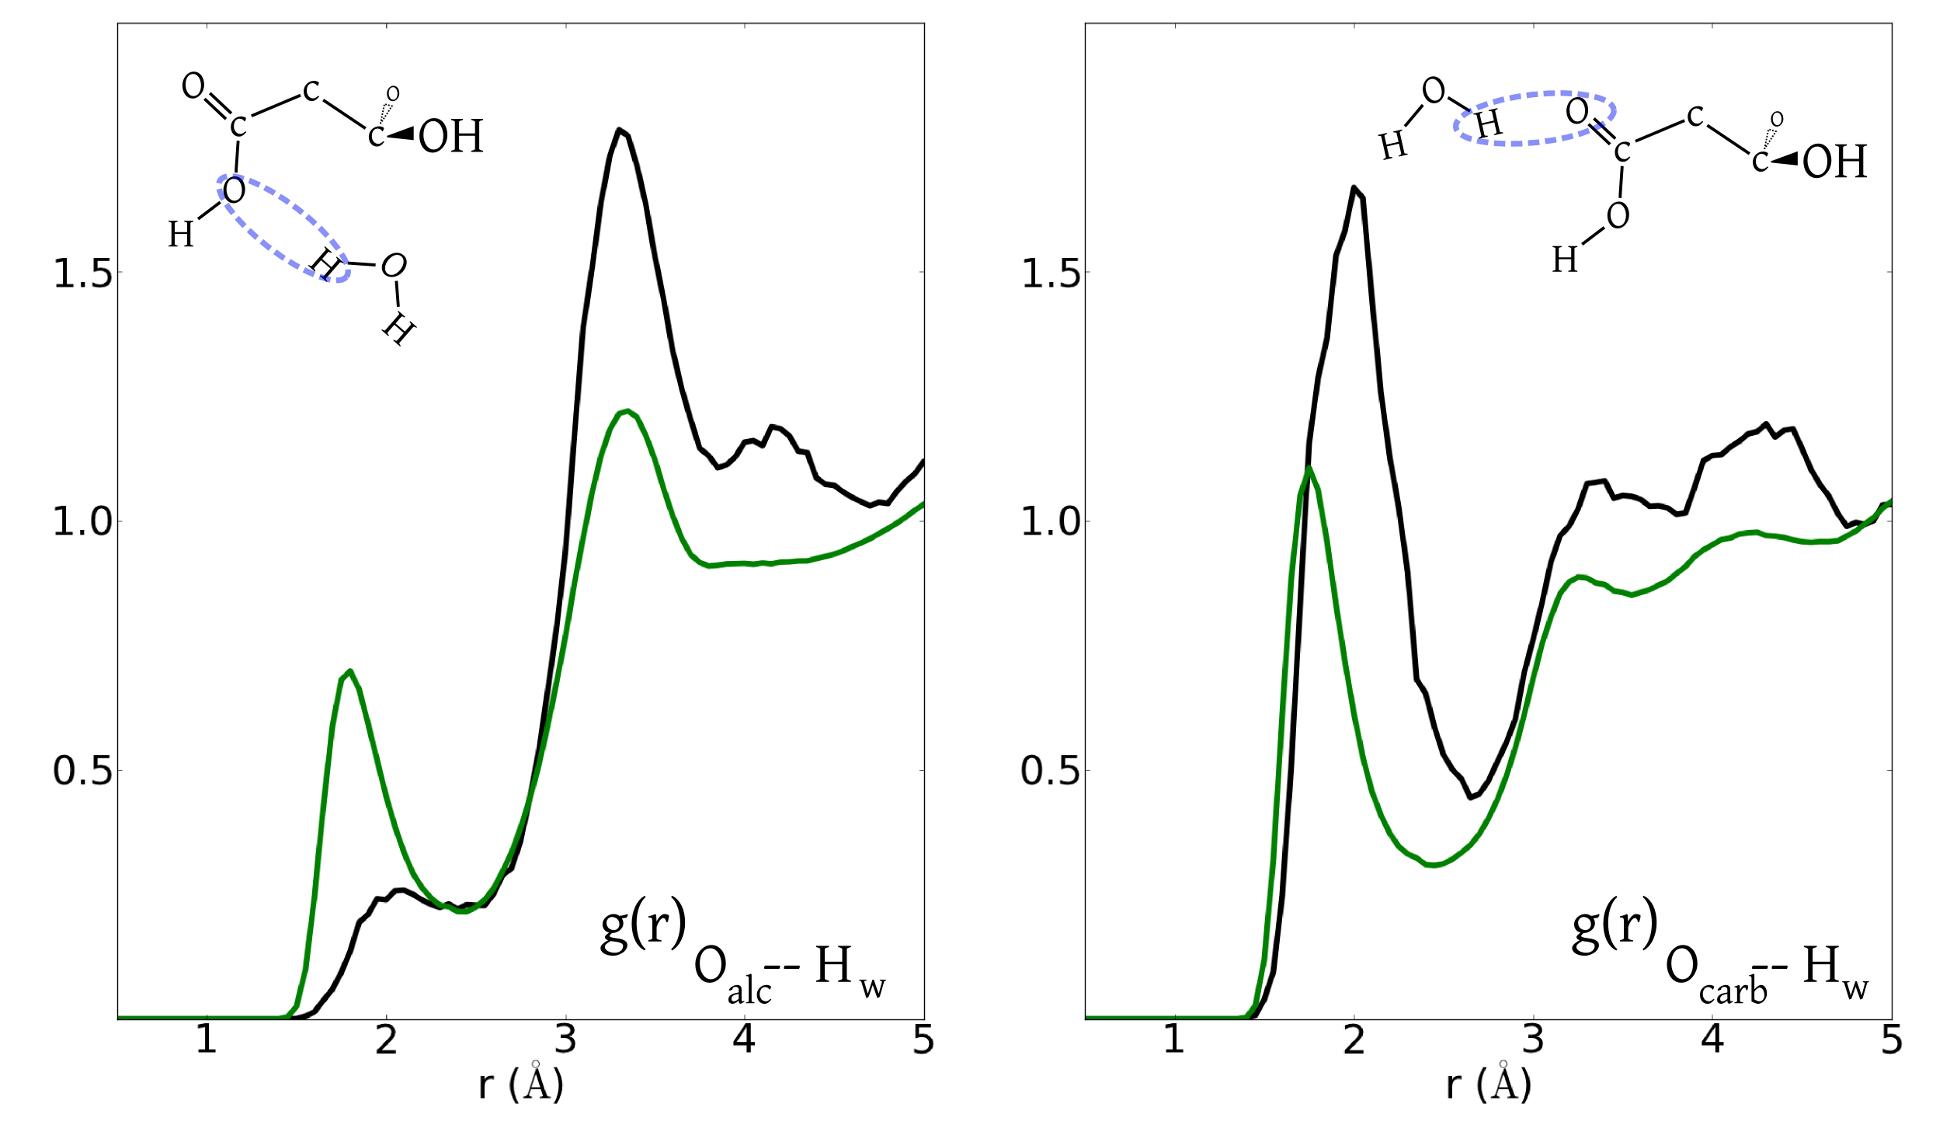
\includegraphics[scale=1.0]{images/rdf/MalonicRDF-small.png}
		\caption{Radial distribution functions, g(r), were calculated for the pair correlations between the acid oxygens and water hydrogen atoms. The acid alcohol moiety oxygen - water hydrogen RDF (left) and the carbonyl oxygen - water hydrogen RDF (right) are plotted. Each RDF is shown for both the KS-DFT simulations of the present study (black), and for classical MD simulations (green) taken from a data set used for a recently published study by our group.\cite{Blower2012}}
		\label{fig:rdf}
	\end{center}
\end{figure}

\section {Molecular Orientation}

Hydration of malonic acid by surface waters and its resulting internal geometry strongly affect the acid's surface behavior. A change in the water environment around the acid can strongly alter the overall orientation of the molecule with respect to the water interface. In the following analysis we examine molecular orientation of malonic using a set of angles to define how the molecule orients in space at an aqueous interface, and how the acid groups orient internally in the molecule. For a complete discussion of the angles used in our analysis, we refer the reader to our previous publication that fully defines them.\cite{Blower2012}

Here we briefly introduce the angles used in the analysis, and provide a graphical depiction of their definitions in Figure \ref{fig:angle-definitions} for reference. We define the overall molecular orientation by the configuration of the three carbon atoms that form the acid's backbone. Two angles, $\theta$ and $\phi$, describe the carbon backbone ``tilt'' and ``twist'', respectively. The tilt angle, $\theta$, is measured from a reference axis (herein defined as the vector normal to the plane of the water interface) to the carbon-group bisector axis (bisecting the two C-C bonds, and pointing from the central carbon towards the direction of the other two carbon atoms). The backbone twist, $\phi$, is rotation of the carbon group about the bisector axis. If the bisector lies in the plane of the water interface such that \thetaeq 90\degr, the twist will have a value of \phieq 0\degr~when the plane of the three carbons is perpendicular to the plane of the water surface. A combination of \thetaeq 90\degr~and \phieq 90\degr~indicates an orientation with the plane of the carbon group lying flat to the plane of the water surface.

Furthermore, we are able to orient the carboxylic acid moieties in the molecule by quantifying the dihedral angle, $\psi$, for each of the two acid groups. The angle $\psi$ is a rotation of the plane of the O=C-O atoms of a carboxylic acid group relative to the plane of the three carbon atoms. An orientation aligning the carbonyl bond vector (pointing from C to O) of a carboxylic acid group parallel to the carbon group bisector results in a dihedral of \psieq 0\degr. Depictions of the angle definitions, and various values of $\psi$ for one of the carboxylic acid groups, are shown in Figure \ref{fig:angle-definitions} for reference.

Plots of the \thetaphi~distributions are provided in Figure \ref{fig:theta-phi}. Three bivariate histograms are shown, depicting the orientational trends of the carbon backbone group. In these intensity plots, high intensity regions are colored darker red, and low intensity is colored dark blue. Regions of the plots exhibiting uniform coloration indicate isotropic behavior, whereas concentrated regions of high intensity show a preference for a particular orientation given by the specific angle combinations.

The larger plot on the left of Figure \ref{fig:theta-phi} shows the angle distribution collected from the data of all five simulations. The highest intensity region is centered at \thetaeq 135\degr, and \phieq 90\degr. This indicates an orientation of the carbon backbone group tilted 45\degr~from the plane of the water surface with the central carbon further out towards the gas-phase side of the interface than the two carbonyl carbons. Additionally, the $\phi$ values show that the two carbonyl carbons are both at similar depths into the water side of the interface.

Although the entire range of $\theta$ and $\phi$ values are represented in the distribution, the bulk of the intensity is concentrated around \thetaeq 135\degr, and very little intensity appears below \thetaeq 90\degr. Thus, there is a clear orientational preference established for the carbon group atoms, and this has a direct effect on the orientation of the other atoms in the molecule.

These orientational results complement those found in our previous classical force field simulation study of malonic acid.\cite{Blower2012} In that study the behavior of the top-most malonic acid molecules on a water surface exhibited a very similar \thetaphi~distribution as in the results shown in Figure \ref{fig:theta-phi}. However, acids located deeper into the water bulk of the classical simulations reoriented, showing interfacial layers of orientational preference that changed with depth. In the present work, only the top-most acids on a water surface are examined, as none of the simulated molecules moved deeper into the water side of the interface.

The results of the \thetaphi~analysis were further broken down to expose differences between the internally unbonded, and intramolecularly hydrogen bonded systems, with results plotted on the top-right and bottom-right of Figure \ref{fig:theta-phi}, respectively. Those systems without the internal H-bonded malonic acid exhibit a very strong orientational preference in $\theta$. The internally unbonded set of acids are entirely oriented with $\theta >$ 90\degr, and the orientational distribution is tightly concentrated around \thetaeq 135\degr. The twist, $\phi$, is concentrated around a value of approximately \phieq 75\degr, with a smaller high-intensity region at $\phi >$ 80\degr. As the twist angle decreases from 90\degr~the two ends of the carbon atom chain move to different depths in the interface. Upper values of $\phi$ in the most intense region of the distribution reach near \phieq 60\degr, resulting from a twist that sends one end of the molecule 30\degr~further out of the aqueous surface than the other. The internally unbonded acids are thus more likely to experience slightly different solvation environments at either end of the molecule if one end is further away from surface waters.

Turning now to the intramolecularly bonded malonic acid \thetaphi~plot of Figure \ref{fig:theta-phi}, we see slightly different orientational preferences. The region of highest intensity is concentrated at \phieq 90\degr, and spread over a wide range of $\theta$, approximately between 90\degr $< \theta <$150\degr. Furthermore, $\theta$ values in the plot span the entire range down to \thetaeq 0\degr. Clearly the intramolecular bonding leads to greater orientational freedom as evidenced by the less concentrated distribution and greater range of orientations. This is intuitively expected for a molecule that has less bonding to neighboring waters due to an internal hydrogen bond occupying both carboxylic acid functional groups. Water is less likely to interact with a malonic acid that has fewer binding sites, and will not stabilize the acid's position or orientation as much as in the internally unbonded case. Thus, the internal H-bond frees the acid molecule to take many more orientations on the water surface than the counterpart internally unbonded acid.

The internal geometry of malonic acid is defined here by the two dihedral angles that quantify rotations of the carboxylic acid groups about the molecule's two C-C bonds. As mentioned earlier, the angle $\psi$ is referenced by the alignment of the C=O carbonyl bond with the C-C-C group bisector. Figure \ref{fig:angle-defintiions} depicts various orientations of a carboxylic acid group and the accompanying value of $\psi$. The overall \psipsi distribution is plotted on the left of Figure \ref{fig:psi-psi} with the plots of the internally unbonded and hydrogen bonded systems to the right in the figure on top and bottom, respectively. The larger plot of all simulation data is overwhelmed by the high intensity concentration at the \psipsi region of 0\degr-180\degr~at the bottom left of the plot. Much lower intensity regions appear throughout the \psipsi range.

Looking to the intramolecularly bonded plot at the bottom right of Figure \ref{fig:psi-psi} it is clear why the larger plot of all the data sets is similarly concentrated at the bottom left of the plot. All of the intensity of the internally bonded acids indicates that the two carbonyl C=O bonds are aligned anti-parallel to each other. The strong H-bond holds the internal geometry nearly fixed with very little distortion through bending of the acid's six-member atom ring structure that forms with the added hydrogen bond interaction. An intense and highly concentrated region of the dihedral angle distribution is thus expected for the stable and mostly rigid form of the internally bonded malonic acid.

The internally unbonded malonic acids exhibit a very different behavior in their carboxylic acid orientations. The top-right plot of Figure \ref{fig:psi-psi} shows the much broader, less concentrated distribution resulting from acids without the internal H-bonding constraints. The multiple regions of low intensity throughout the plotted range speak to the molecule's much greater flexibility, and the nature of having the two carboxylic acid ends of the molecule much more decoupled. However, a trend is apparent in the distribution of the two dihedral angles. There appears to be two regions in the plot located at the center-left and top-center of the plot. In our previously published results of the complementary classical force field simulations,\cite{Blower2012} the \psipsi distributions throughout the interfacial region had two similarly located peaks. In that study the regions of the plot were more concentrated over small areas at \psipsi values of 0\degr~and 90\degr. That combination is indicative of the dihedrals aligning 90\degr~from each other, i.e. perpendicularly. One of the C=O bonds is aligned parallel to the C-C-C bisector (\psieq 0\degr), and the other is perpendicular to the plane formed by the C-C-C atoms (\psieq 90\degr). The correspondence of the two regions in the distribution of the present work to those of the classical simulations is noteworthy The classical force field reproduces the dihedral trend of two peaks in the distribution, but the much smaller region over which the $\psi$ angles appear suggests that the corresponding term in the classical potential needs to be adjusted to better recreate the ab initio results for higher accuracy. The present results, however, suggest that without further modifications, there is good agreement between the ab initio and classical potentials with regards to the overall orientation of surface malonic acid molecules. The shortcoming of the classical potential is its inability to properly capture the internal hydrogen bond conformation. Though, that conformation may not be a major overall contributor to the distribution of acids found at a water surface.

% theta_{C=O}
Having now established the \thetaphi orientational trend of the carbon backbone atoms, and the \psipsi dihedral relationships, we have a nearly complete orientational picture of surface malonic acid. What remains to determine is the absolute orientation of both carboxylic acid groups with respect to the plane of the water surface. In order to compare the orientational results with our recent experimental results determined by the SFG spectra of the carbonyl modes of malonic acid,\cite{Blower2012} we now further expand on the configuration of the carboxylic acid groups. Specifically, the analysis presented shows how the carbonyl C=O bond vectors orient relative to the reference axis normal to the plane of the interface, forming a new angle, \thetacarb.

The distribution of \thetacarb is presented in Figure \ref{fig:theta-carb}. The black plot shows the distribution of angles from all simulation datasets. The red and blue plots correspond to the \thetacarb data collected only from the intramolecularly H-bonded, and internally unbonded simulations, respectively. In all the distributions two angle regions dominate in population, appearing as peaks from approximately 50\degr-120\degr, and 150\degr-180\degr. The former angle range corresponds to carbonyl C=O bonds pointing in the plane of the water surface ($\theta_{C=O}=90$\degr~indicates a carbonyl parallel to the plane), slightly above, or slightly below the plane. The latter range indicates carbonyl bonds pointing directly in towards the water side of the interface ($\theta_{C=O}=180$\degr) or within a cone of approximately 30\degr~tilt from the reference axis into the water bulk.

Looking at the individual red and blue plots, there are some differences between how the acid internal bonding conformations behave. The lower peak of the blue plot is centered at approximately $\theta_{C=O}=90$\degr, with a peak width extending up to 30\degr~to either side. The peak near 180\degr~is slightly broader down to 130\degr. Between the two peaks there is a small baseline population, whereas for $\theta_{C=O} < 50$\degr, there is very little or no distribution height.

The red plot, representing the intramolecularly H-bonded acids, is overall lower in magnitude than the blue plot because only two of the five simulations are represented. Additionally, there is a persistent population throughout the entire \thetacarb range, as compared to the blue plot that disappears at the lower angles. The location of the lower peak is centered near $\theta_{C=O}=70$\degr, which is almost 20\degr~lower than the equivalent blue distribution peak. The width of the red peak is smaller, spanning approximately 20\degr~less angle range. The peak at 180\degr~is similarly narrower by nearly 20\degr.

In both sets of simulations there is a clear trend for malonic acid to point one of the carbonyl bonds into the water side of the interface ($\theta_{C=O}=180$\degr), and the other bond points in the plane of the interface, or slightly above of below it ($\theta_{C=O} \approx 90$\degr). The formation of the internal H-bond slightly shifts the angle of the more in-plane carbonyl to point further out away from the water side of the interface. Also, the internally bonded acids enjoy a greater orientational freedom in their carbonyls overall (i.e. the distribution has population throughout all angle regions), but the peaks in the distribution are narrower than for the internally unbonded molecules. It is likely that the orientation of the carbonyl bonds on the water surface will affect their solvation environments, and their consequent hydration by surface waters. The internally H-bonded malonic acid has a peak in the distribution of \thetacarb that lies slightly further to the left (i.e. lower angle values) than its unbonded counterpart. Lower angle values indicate a carbonyl bond tilt further out from the surface, away from the water bulk. This slight orientational difference likely leads to a difference in the strength or amount of hydration on this particular carbonyl bond. The effect of this will become apparent spectrally, and may lead to interesting chemical differences between the two conformations.

\section {Bond Spectra}

Knowing the orientational behavior of malonic acid helps us to establish a model for how the molecule behaves on an aqueous surface. To link this computationally derived model to our group's experimental work, we turn to the computed spectra of one of the functional moieties of the acid molecules. The bondlengths of the carbonyl C=O bonds were calculated for each simulation at each timestep (similar to the results presented earlier in Figure \ref{fig:bondlength-trajectory}) to generate a time-dependent function, $f(t)$. A calculation was then performed on the time function generate the power spectrum of the bond lengths,\cite{BuchPaper,Etc} hereafter referred to as a ``bond spectrum''. While not fully encapsulating the response of dipole transition moments or recreating IR or SFG spectra, the frequencies captured in a bond spectrum are representational of the local mode frequencies expected from experimental spectroscopic studies, and are directly comparable.

Figure \ref{fig:bond-spectra} shows the C=O carbonyl bond spectrum averaged from all the simulations (top, black spectrum). The two colored spectra in Figure \ref{fig:bond-spectra} show the contributions of the intramolecularly H-bonded and internally unbonded malonic acids, in the bottom and middle spectra, respectively. The coloration of the bottom two plots matches that of Figure \ref{fig:bondlength-distribution}, where the spectral contribution of the carbonyl taking part in the internal H-bond is colored maroon, and the other carbonyl bond response is colored yellow. The color-coded graphic of the molecule for both internal bonding conformations has been reproduced for reference. For the internally unbonded malonic acids, the coloring is more arbitrarily assigned because of the interchangeability of the two bonds.

The top spectrum of Figure \ref{fig:bond-spectra} spans approximately 130\cm, with a maximum located towards the upper frequencies near 1700\cm. The width of the spectrum suggests a large distribution of solvations environments in which the carbonyl bonds are interactinve with surface waters. In our previous SFG spectroscopic experiments, the response of surface malonic acid molecules was determined to lie within the same spectral range, with peaks centered at ???\cm and ???\cm. The experimental results are very well reproduced in these bond spectra calculations, increasing confidence in the computational method employed for the simulations, and also the consequent picture developed for the orientation and other behaviors of the acid molecules.

To further emphasize the differences between the internally H-bonded and unbonded configurations of malonic acid, the bottom two spectra of Figure \ref{fig:bond-spectra} show the contributions of each set of simulations. The internally unbonded acids have the two ends of the molecule acting more independently than with the internal bond. The two carbonyls can thus both experience a full range of solvations environments. The spectral response of these two carbonyls are expected to be similar, or overlapped in frequencies. As shown in the middle spectrum of Figure \ref{fig:bond-spectra}, the two carbonyl spectra are mostly overlapped, and form the central contributions to the overall spectrum from the collection of all simulation datasets (top of Figure \ref{fig:bond-spectra}). Looking to the bottom spectrum in Figure \ref{fig:bond-spectra}, there is a dramatic splitting of the two carbonyl peaks. The C=O bond involved in the intramolecular H-bond is red-shifted, and the other carbonyl is blue-shifted compared to the internally unbonded spectra. This shift in frequencies shows the strong effect of an internal H-bond on both the bonded carbonyl, and the outter uninvolved carbonyl bond.

In this study, the statistical distribution of the two internal bonding conformations could not be established because of the limited data collected and computational resources used. Thus, the intensities of the spectra can not be directly compared to experimental results, but the frequencies themselves are representational of those for carbonyl bonds. Future studies employing more statistically complete data sets will likely further establish the spectral response of these surface-hydrated malonic acids. Furthermore, it will be possible to establish wether the intramolecularly H-bonded conformation is a statistically relevant species at aqueous surfaces. However, it is possible to conclude that the highest and lower frequency carbonyl responses are contributed by malonic acids with specific geometric conformations (e.g. internal bonding), or some other form of solvation that constrains the motions and interactions of the acid.

\section {Conclusions}

The adsorption of small organic and chemically active molecules has gained great interest in recent years. Understanding their reactivities, orientations, adsorption pathways, and surface behaviors is of primary concern in building accurate atmospheric climate models, and in defining the many aqueous environments found on earth. Yet, the specific microscopic nature of such organics, their surface geometries, orientations, and water interactions remain poorly understood. Although our comprehension of surface processes and interfacial chemistry is still in its infancy, we are beginning to gain new insights that are key to understanding environmentally important processes at aqueous surfaces.

Presented herein are results of KS-DFT MD simulations that focus on how malonic acid behaves on a water surface, and the resulting orientations, geometries, and structures formed because of its interactions with interfacial water molecules. This computational study complements and expands on experimental studies from this laboratory that elucidated the molecular behavior of malonic acid.\cite{Blower2012} Furthermore, these computations build upon and enhance our understanding of malonic acid from the computational study on interfacial orientation and geometry of aqueous surface malonic acid molecules.

Our simulations show that the previously used classical interaction potential captures the orientation and hydration structure of the KS-DFT model. The complementary simulations studies using both interaction potentials show strong agreement for the surface-bound malonic acid behaviors. However, the classical model does not fully capture the resonance structures of the carboxylic acids, leading to minor discrepancies between the water structures that form to hydrate the acids.

Our analysis of intramolecular atomic distances resulted in the discovery of two dominant conformations of surface malonic acid: an intramolecularly hydrogen-bonded species, and an acid in which neither carboxylic acid end-group takes part in internal bonding. The hydrogen bonded structure forms a ring-like internal geometry due to the folding of one carboxylic acid end towards the other, and subsequent hydrogen-bonding. The internal H-bond is strong and persistent throughout 40 ps of simulation, and warrants further experimental study to verify the existence of the species. The distribution of bondlengths in the surface malonic acid indicate that the two conformations of the acid have non-equivalent carboxylic acid moieties. In the hydrogen-bonded form, the bondlengths in one carboxylic acid end of the molecule differ from those at the other end. Delocalization of the atoms involved in the hydrogen bond causes elongation of the interacting bonds. The bondlengths and molecular geometry are accompanied with orientational and spectral changes brought on by the internal bonding of the molecule.

We have shown the results of an orientational analysis defining the overall molecular orientation of malonic acid on a water surface, and the configuration of the two carboxylic acids. The carbon backbone was found to lie slightly tilted from the plane of the interface. The hydrogen-bonded conformation has much more orientational freedom than its unbonded counterpart. Analysis of the dihedral angles of the carboxylic acids showed two distinct trends dependent on the specific molecular bonding conformation. The internally unbonded molecule's carboxylic acids orient very similarly to those found in our previous computational study, with one aligning perpendicular to the other. However, the internally H-bonded acid has a very defined internal orientation, with one carbonyl aligned anti-parallel to the other due to a rigid backbone structure reinforced by the intramolecular bonding.

The orientation of the carbonyl bonds was analyzed to complete the picture of the molecular orientation of surface malonic acid. Two distinct carbonyl C=O behaviors were found to be preferred, with one C=O bond pointing more in the plane of the water surface, and the other pointing more perpendicularly, in towards the water bulk. This result agrees well with our previous classical simulation results, and also complements the conclusions from our VSFS experiments showing two preferred net orientations of the carbonyl C=O modes. As with the other computational results, the H-bonded form has greater orientational freedom overall for the carbonyl C=O bonds.

Lastly, to compare the KS-DFT vibrational modes with experiment, the local mode bond spectra were calculated for the carbonyl C=O bonds. The frequencies and spectral shape agree with what we found experimentally via VSFS of the surface-bound C=O modes. Although direct comparison of the spectra is not possible, the resulting frequency range reinforces the predictions of our simulations. Additionally, the C=O spectra of the internally H-bonded conformation show a splitting of the two C=O modes because of the drastically different environments surrounding each bond.

These studies build upon our computational and experimental research in this area, seeking to understand how small organic molecules behave while bound to, and reacting with an aqueous/air interface. Such knowledge is our key to understanding atmospheric aerosol and land water systems where small and reactive organic acid molecules bind to aqueous surfaces, and form platforms for further chemical reactions. Further studies of these systems will aid us in better understanding water surfaces where molecular behavior can surprise us, and often defies our physical intuitions.


\bibliography{malonic-study}

\end{document}
